\documentclass[8pt]{beamer}

\newif\ifplacelogo % create a new conditional
\placelogotrue % set it to true

\usetheme{Warsaw}
\usecolortheme{rose}
\usepackage{multicol}
\usepackage{epstopdf}
\usepackage[italic]{hepnames}
\usepackage{tikz}
\usepackage{listings}
\usepackage{times}
\usepackage{amsmath}
\usepackage{verbatim}
\usepackage{hyperref}
\usepackage{bbding}
\usepackage{upgreek}
\lstset{breakatwhitespace,
language=C++,
columns=fullflexible,
keepspaces,
breaklines,
tabsize=3, 
showstringspaces=false,
extendedchars=true}

% TikZ includes!!!
\usepackage{tikz}
\usetikzlibrary{backgrounds}
\usetikzlibrary{calc}
\tikzstyle{every picture}+=[remember picture]
\input{/home/oviazlo/Desktop/beamerPresentations/myReports/latexHelpScripts/tikzGrid.tex}


\begin{document}

% custom colors
\definecolor{olive}{rgb}{0.3, 0.4, .1}
\definecolor{fore}{RGB}{249,242,215}
\definecolor{back}{RGB}{51,51,51}
\definecolor{title}{RGB}{255,0,90}
\definecolor{dgreen}{rgb}{0.,0.6,0.}
\definecolor{gold}{rgb}{1.,0.84,0.}
\definecolor{JungleGreen}{cmyk}{0.99,0,0.52,0}
\definecolor{BlueGreen}{cmyk}{0.85,0,0.33,0}
\definecolor{RawSienna}{cmyk}{0,0.72,1,0.45}
\definecolor{Magenta}{cmyk}{0,1,0,0}

\definecolor{PixelColor}{RGB}{207,232,139}
\definecolor{SCTColor}{RGB}{167,166,255}
\definecolor{TRTColor}{RGB}{250,224,140}
\definecolor{grayColor}{RGB}{153,153,153}

\newcommand{\yRefPosOne}{0.0}
\newcommand{\xRefPosOne}{0.0}
\newcommand{\yRefPosTwo}{0.0}
\newcommand{\xRefPosTwo}{0.0}
\newcommand{\yRefIncrementOne}{0.0}
\newcommand{\xRefIncrementOne}{0.0}
\newcommand{\yRefIncrementTwo}{0.0}
\newcommand{\xRefIncrementTwo}{0.0}

\graphicspath{ {/home/oviazlo/Desktop/beamerPresentations/FCCee/pictures/plots_CALICE_workshop/} }


\DeclareGraphicsExtensions{.eps, .pdf, .png}

\newcommand{\myBox}[2][pink] {
    \noindent\colorbox{#1}{
	\textbf{#2}
    }\par
}

% For nice block (provided by Oleh)
\tikzstyle{myBox} = [draw=red, fill=blue!1, very thick,
    rectangle, rounded corners, inner sep=5pt, inner ysep=9pt]
    
\tikzstyle{PixelBox} = [draw=PixelColor, fill=blue!1, very thick,
    rectangle, rounded corners, inner sep=5pt, inner ysep=9pt]
\tikzstyle{SCTBox} = [draw=SCTColor, fill=blue!1, very thick,
    rectangle, rounded corners, inner sep=5pt, inner ysep=9pt]
\tikzstyle{TRTBox} = [draw=TRTColor, fill=blue!1, very thick,
    rectangle, rounded corners, inner sep=5pt, inner ysep=9pt]

% poster advertisement
\newcommand{\myCenterBox}[2][pink] {
   {\centering
    \noindent\colorbox{#1}{
	\textbf{#2}
    }\par
  }
}

\newcommand{\mySmallCenterBox}[2][pink] {
   {\centering
    \noindent\colorbox{#1}{
	\textbf{{\small #2}}
    }\par
  }
}

\newcommand{\myVerySmallCenterBox}[2][pink] {
   {\centering
    \noindent\colorbox{#1}{
	\textbf{{\scriptsize #2}}
    }\par
  }
}

\newcommand{\backupbegin}{
   \newcounter{finalframe}
   \setcounter{finalframe}{\value{framenumber}}
}
\newcommand{\backupend}{
   \setcounter{framenumber}{\value{finalframe}}
}

\newcommand{\myNode}{\tikz[baseline,inner sep=1pt] \node[anchor=base]}

\tikzstyle{fancytitle} =[fill=white!15, text=black]

\definecolor{light-gray}{gray}{0.95}
% poster advertisement


\title[ CLD detector model overview \hspace{13.5em}\insertframenumber/
\inserttotalframenumber]{ CLD detector model overview}


	\author[Oleksandr Viazlo]{Oleksandr Viazlo \\ 
% 	{\small ???}
	}
	\institute{\small CERN\\} 
	
       
	\date{4 April 2018}

% 	\logo{ \ifplacelogo \includegraphics[height=1.8cm]{./ID_week2/lund_uni-logo_s.pdf} \hspace{0.4cm} \fi}

	
   	\frame{\titlepage}

   	

\placelogofalse

% %*****************************************************************************
% \begin{frame}
% \frametitle{Introduction} 
% 
% \renewcommand{\yRefPosOne}{0}
% \renewcommand{\xRefPosOne}{5.3}
% \renewcommand{\xRefIncrementOne}{5.5}
% 
% \begin{tikzpicture}[overlay]
% 
% 
% %% HELPER draw advanced helping grid with axises:
% % \draw(-0.5,-4) to[grid with coordinates] (11.5,4);
% 
% \end{tikzpicture}
% \end{frame}
% %*****************************************************************************
% %*****************************************************************************
% \begin{frame}{}
%     \begin{tikzpicture}[overlay]
%     \node[right] (textNode) at (3.5,0) {
%       {\large \bf CLD Detector Model}
%     };
%     \end{tikzpicture}
% \end{frame}
% %*****************************************************************************
%*****************************************************************************
\begin{frame}{\large \large CLD detector model}

\renewcommand{\yRefPosOne}{0}
\renewcommand{\xRefPosOne}{5.3}
\renewcommand{\xRefIncrementOne}{5.5}
\begin{tikzpicture}[overlay]

 \node[inner sep=0pt] (tmp) at (\xRefPosOne-2.15,\yRefPosOne-0.56)
    {\includegraphics[width=7.8cm]{../CEPC_workshop/FCCeePictsFromKonrad/CLIC_FCC_Top_QuarterView_withLabes.png}};

\node  at (\xRefPosOne,\yRefPosOne+2.8) (box){%
\myCenterBox{\small CLD model}
}; 
    
    \draw[black, thick, ->] (-0.8,-4.76)--(-0.8,3.7) node[pos=0.95, right]{\small R [m]};
    \draw[black, thick, ->] (-0.8,-4.76)--(6.5,-4.76) node[pos=0.95, below]{\tiny Z [m]};
    
  \node[inner sep=0pt] (tmp) at (\xRefPosOne-3.05,\yRefPosOne-4.9)
    {2.3};   
  \node[inner sep=0pt] (tmp) at (\xRefPosOne-1.14,\yRefPosOne-4.9)
    {3.7};  
    
%     \node [PixelBox] at (\xRefPosOne+3.7,\yRefPosOne-4) (box){%
%   \begin{minipage}{0.43\textwidth}
%     Detector design inspired by detectors for CLIC and ILC and optimized for FCC-ee conditions
%   \end{minipage}
% };

\node [PixelBox] at (\xRefPosOne+3.7,\yRefPosOne+2.5) (box){%
  \begin{minipage}{0.43\textwidth}
    CLD detector model is inspired by detectors for CLIC and ILC and optimized for FCC-ee conditions
  \end{minipage}
};

\node  at (\xRefPosOne+3.5,\yRefPosOne-1.5) (box){%
    \begin{minipage}{0.5\textwidth}

  \begin{itemize}
      \item Full silicon tracking system - provides $\geqslant$12 hits per track 
      \item 2 T magnetic field (constrains from the machine) $\to$ 2.1 m large tracker radius \\[0.4cm]
      \item Fine-grained ECAL and HCAL optimised for particle flow reconstruction \\[0.4cm]
      \item Superconducting solenoid is outside of calorimeter \\[0.4cm]
      \item Steel return yoke with muon chambers\\[0.4cm]
   
   \item Forward detector region ($<$ 150 mrad) is reserved for Machine-Detector Interface (accommodates LumiCal)
%    : \\ MDI region 
%    (accommodates LumiCal)
   \\[0.3cm]
  \end{itemize}

    \end{minipage}
};







% \node [PixelBox] at (\xRefPosOne+3.7,\yRefPosOne-4) (box){%
%   \begin{minipage}{0.43\textwidth}
%     Detector design inspired by detectors for CLIC and ILC and optimized for FCC-ee conditions
%   \end{minipage}
% };

%% HELPER draw advanced helping grid with axises:
% \draw(-0.5,-4) to[grid with coordinates] (11.5,4);
\end{tikzpicture}

 
\end{frame}
%*****************************************************************************
%*****************************************************************************
\begin{frame}{\large \large Tracking system}

\renewcommand{\yRefPosOne}{0}
\renewcommand{\xRefPosOne}{5.3}
\renewcommand{\xRefIncrementOne}{5.5}
\begin{tikzpicture}[overlay]

\node[PixelBox] (tmp) at  (\xRefPosOne-3.2,\yRefPosOne+1.7) (box){%

  \begin{minipage}{0.46\textwidth}
    \begin{itemize}
     \item Silicon pixels: 25x25$\upmu$m
     \item Single-point resolution: 3 $\upmu$m
     \item 3 double layers in barrel: \\17-57 mm
     \item 3 double endcap disks per side: 160 - 300 mm
     \item Material budget: 0.3$\%$ X$_0$ per layer
    \end{itemize}

  \end{minipage}
};
\node[fancytitle, right=15pt] at (box.north west) {Vertex detector};

\node[TRTBox] (tmp) at  (\xRefPosOne-3.2,\yRefPosOne-2.3) (box){%

  \begin{minipage}{0.46\textwidth}
    \begin{itemize}
     \item Silicon pixel and microstrips detector
     \item Inner Tracker:
     \begin{itemize}
      \item 3 barrel layers, 7 disks
     \end{itemize}
     \item Outer Tracker:
     \begin{itemize}
      \item 3 barrel layers, 4 disks
     \end{itemize}
     \item Single-point resolution:
     \begin{itemize}
      \item 7 $\upmu$m x 90 $\upmu$m
      \item except 1st IT disk: 5 $\upmu$m x 5 $\upmu$m
     \end{itemize}
     \item Material:  1.1-1.6$\%$ X$_0$ per layer
%      \item Material budget: 
%      \begin{itemize}
%       \item barrel: 1.1-1.2$\%$ X$_0$ per layer
%       \item disks: 1.4-1.6$\%$ X$_0$ per layer
%      \end{itemize}

     
    \end{itemize}

  \end{minipage}
};
\node[fancytitle, right=15pt] at (box.north west) {Tracker detector};

% \node[PixelBox, inner sep=2pt] (tmp) at  (\xRefPosOne+2,\yRefPosOne+1.3) (box){%
\node[inner sep=0pt] (tmp) at  (\xRefPosOne+2.8,\yRefPosOne-3.1) (box){%
% \node[inner sep=0pt] (tmp) at  (\xRefPosOne+2.5,\yRefPosOne+1.3) (box){%
    {\includegraphics[width=5cm]{/home/oviazlo/Work/Note_FCCeeDetector/figures/Sasha_17Jan2018_materialBudget_FCCee_o1_v02.pdf}}
};
% \node[fancytitle, right=5pt] at (box.north west) {VTX + Tracker + Beampipe Material Budget};
    
\node (tmp.west) at  (\xRefPosOne+3.9,\yRefPosOne-4.0) (box){%
  \begin{minipage}{0.44\textwidth}
   VTX + Tracker + Beampipe \\Material Budget
  \end{minipage}
};
    
\node[inner sep=0pt] (tmp) at  (\xRefPosOne+3.0,\yRefPosOne+1.3) (box){%
% \node[inner sep=0pt] (tmp) at  (\xRefPosOne+2.8,\yRefPosOne-2.6) (box){%
    {\includegraphics[width=5cm]{/home/oviazlo/Work/Note_FCCeeDetector/figures/full_Tracker_FCCee_probe_v2.pdf}}
};

% \node[TRTBox] (tmp.west) at  (\xRefPosOne-3.2,\yRefPosOne-2.3) (box){%
% 
%   \begin{minipage}{0.46\textwidth}
%    fds dsf 
%   \end{minipage}
% };
    
    \node  at (\xRefPosOne-2.7,\yRefPosOne-4.7) (box){%
      \myCenterBox{\small Support structures, cables and services are included}
    };     
    
% \node  (tmp.west) at (\xRefPosOne-0.5,\yRefPosOne-4.7) (box){%
%     \begin{minipage}{\textwidth}
% 
%     {
%     Support structures, cables and services are included
%     }
% %   \begin{itemize}
% %    \item ???
% % \end{itemize}
% 
%     \end{minipage}
% };
    
    
%% HELPER draw advanced helping grid with axises:
% \draw(-0.5,-4) to[grid with coordinates] (11.5,4);  
\end{tikzpicture}

 
\end{frame}
%*****************************************************************************
%*****************************************************************************
\begin{frame}{\large \large Calorimetry}

\renewcommand{\yRefPosOne}{0}
\renewcommand{\xRefPosOne}{5.3}
\renewcommand{\xRefIncrementOne}{5.5}
\begin{tikzpicture}[overlay]

\node[inner sep=0pt] (tmp) at  (\xRefPosOne+2.5,\yRefPosOne-3.2) (box){%
    {\includegraphics[width=4.5cm]{/home/oviazlo/Work/Note_FCCeeDetector/figures//Sasha_15Mar2018_nuclearInteractionLengthsCalorimeter_FCCee_o1_v02.pdf}}
};

\node[inner sep=0pt] (tmp) at  (\xRefPosOne+3.7,\yRefPosOne+0.5) (box){%
    {\includegraphics[width=5.5cm]{/home/oviazlo/Work/Note_FCCeeDetector/figures/calo_overall_view.pdf}}
};




\node[TRTBox, inner sep=7pt] (tmp) at  (\xRefPosOne-3.1,\yRefPosOne-3.8) (box){%
    {\includegraphics[width=5.5cm]{/home/oviazlo/Work/Note_FCCeeDetector/figures/HCAL_schematicDrawning.pdf}}
};
\node[fancytitle, right=15pt] at (box.north west) {HCAL layer layout};

\node[PixelBox] (tmp) at  (\xRefPosOne-3.2,\yRefPosOne+2.0) (box){%

  \begin{minipage}{0.48\textwidth}
    \begin{itemize}
        \item Si-W sampling calorimeter
        \item cell size 5 x 5 mm$^2$
        \item 40 layers (1.9 mm thick W plates)
        \item Depth: 22 X$_0$
    \end{itemize}

  \end{minipage}
};
\node[fancytitle, right=15pt] at (box.north west) {Electromagnetic Calorimeter};

\node[TRTBox] (tmp) at  (\xRefPosOne-3.2,\yRefPosOne-1) (box){%

  \begin{minipage}{0.48\textwidth}
    \begin{itemize}
        \item Scintillator-steel sampling calorimeter
        \item cell size 30 x 30 mm$^2$
        \item 44 layers (19 mm thick steel plates)
        \item Depth: 5.5 $\lambda_I$
    \end{itemize}

  \end{minipage}
};
\node[fancytitle, right=15pt] at (box.north west) {Hadronic Calorimeter};


%% HELPER draw advanced helping grid with axises:
% \draw(-0.5,-4) to[grid with coordinates] (11.5,4);
\end{tikzpicture}

 
\end{frame}
%*****************************************************************************
%*****************************************************************************
\begin{frame}{\large \large The magnet and muon system}

\renewcommand{\yRefPosOne}{0}
\renewcommand{\xRefPosOne}{5.3}
\renewcommand{\xRefIncrementOne}{5.5}
\begin{tikzpicture}[overlay]


\node[PixelBox] (tmp) at  (\xRefPosOne-3.2,\yRefPosOne+1.0) (box){%

  \begin{minipage}{0.43\textwidth}
      \begin{itemize}
     \item 2T superconducting coil outside calorimeter: 
      \begin{itemize}
       \item 90 mm aluminium thick coil
      \end{itemize}

     \item Return yoke (1.5 m thick steel):
     \begin{itemize}
      \item The simulation model assumes 1T field in Barrel and no field in Endcap
     \end{itemize}

    \end{itemize}

  \end{minipage}
};
\node[fancytitle, right=15pt] at (box.north west) {The magnet system};

\node[TRTBox] (tmp) at  (\xRefPosOne-3.2,\yRefPosOne-2.9) (box){%

  \begin{minipage}{0.43\textwidth}


    \begin{itemize}
     \item 6 RPC muon chambers
     \item Cell size: 30 x 30 mm
    \end{itemize}
  
  \end{minipage}
};
\node[fancytitle, right=15pt] at (box.north west) {The muon system};

    
\node[inner sep=0pt] (tmp) at  (\xRefPosOne+2.8,\yRefPosOne-0.6) (box){%
    {\includegraphics[width=7cm]{/home/oviazlo/Work/Note_FCCeeDetector/figures/FCC_clic_muons.pdf}}
};



%% HELPER draw advanced helping grid with axises:
% \draw(-0.5,-4) to[grid with coordinates] (11.5,4);
\end{tikzpicture}

 
\end{frame}
%*****************************************************************************
%*****************************************************************************
\begin{frame}{\large \large Simulation and reconstruction software tools}

\renewcommand{\yRefPosOne}{0}
\renewcommand{\xRefPosOne}{5.3}
\renewcommand{\xRefIncrementOne}{5.5}
\begin{tikzpicture}[overlay]

%  \node[inner sep=0pt] (tmp) at (\xRefPosOne-2.15,\yRefPosOne-0.56)
%     {\includegraphics[width=7.8cm]{FCCeePictsFromKonrad/CLIC_FCC_Top_QuarterView_withLabes.png}};

    
\node  at (\xRefPosOne,\yRefPosOne) (box){%
    \begin{minipage}{\textwidth}

  \begin{itemize}
   \item For performance study of the CLD detector for FCC-ee 
	 one can benefit from the fully functional and well tested \href{https://github.com/iLCSoft}{\color{blue} iLCSoft} software used by the CLIC and ILC community. \\[0.4cm]
   
   \item Detector geometry description and event simulation: \href{https://github.com/AIDASoft/DD4hep}{\color{blue} DD4hep}
   \item Event Reconstruction: \href{https://github.com/iLCSoft/Marlin}{\color{blue} Marlin}\\[0.4cm]
   
   \item Track Pattern recognition: TruthTracking or ConformalTracking
   \item Particle Flow Reconstruction: \href{https://github.com/PandoraPFA}{\color{blue} PandoraPFA} \\[0.6cm]
  
   \item Up-to-date geometry of detector model implemented in lcgeo package: 
   \href{https://github.com/iLCSoft/lcgeo/tree/master/FCCee/compact/FCCee_o1_v02}{\color{blue} FCCee$\_$o1$\_$v02}
%    FCCee$\_$o1$\_$v02

  \end{itemize}

    \end{minipage}
};

\node [PixelBox] at (\xRefPosOne-0.01,\yRefPosOne-3.5) (box){%
  \begin{minipage}{0.99\textwidth}
    Tracking and calorimetry performances have been studied with full detector simulation
  \end{minipage}
};


%% HELPER draw advanced helping grid with axises:
% \draw(-0.5,-4) to[grid with coordinates] (11.5,4);
\end{tikzpicture}

 
\end{frame}
%*****************************************************************************
%*****************************************************************************
% \bgroup
% \setbeamercolor{background canvas}{bg=white}
\begin{frame}{}

    \begin{tikzpicture}[overlay]

    %% HELPER draw advanced helping grid with axises:
%     \draw (0,-5) to[grid with coordinates] (11,3);

    \node[right] (textNode) at (3,0) {
      { \large \bf Tracking performance}
    };
    
    \node[right] (n7) at (4.6,-0.7) {
        \EightStarTaper Momentum and d$_0$ resolutions
    };
    
    \node[right] (n8) at (4.6,-1.2) {
        \EightStarTaper Efficiency for single muons
    };

    \node[right] (n9) at (4.6,-1.7) {
        \EightStarTaper Efficiency in complex events
    };
    
    \tikz[overlay]\draw[thick,black,->] ([xshift=-0.6cm]textNode.south) to [out=270, in=180] ([xshift=-0.1pt]n7.west);
    \tikz[overlay]\draw[thick,black,->] ([xshift=-1.1cm]textNode.south) to [out=270, in=180] ([xshift=-0.1pt]n8.west);
    \tikz[overlay]\draw[thick,black,->] ([xshift=-1.6cm]textNode.south) to [out=270, in=180] ([xshift=-0.1pt]n9.west);    

    \end{tikzpicture}

\end{frame}
% \egroup
%*****************************************************************************
%*****************************************************************************
\begin{frame}{\large \large Momentum and d$_0$ resolutions}
\renewcommand{\yRefPosOne}{-1.5}
\renewcommand{\xRefPosOne}{4.2}
\renewcommand{\xRefIncrementOne}{7.5}
\begin{tikzpicture}[overlay]



 \node[inner sep=0pt] (tmp) at (\xRefPosOne-1.7,\yRefPosOne+0.9)
  {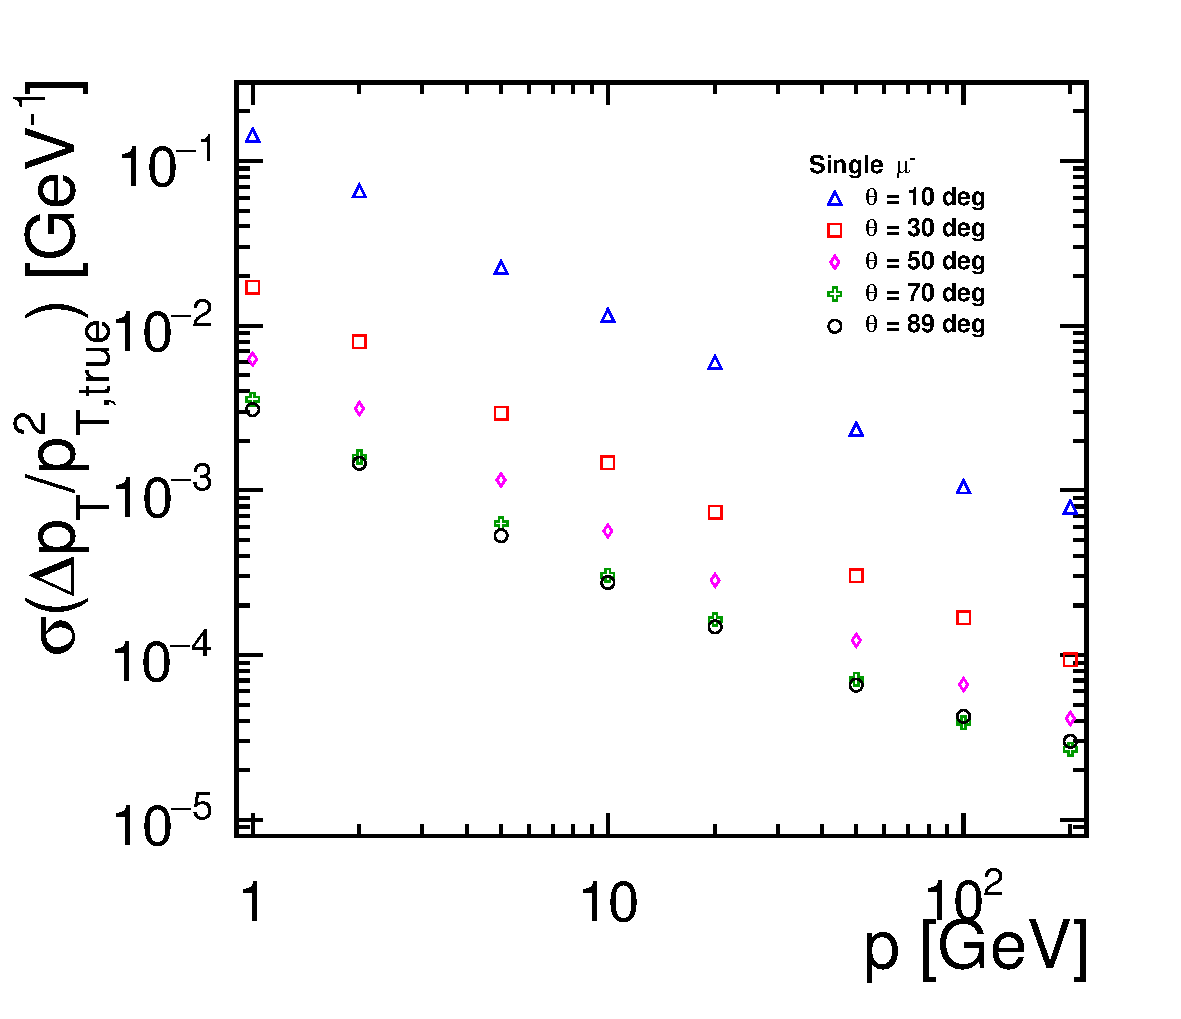
\includegraphics[width=6cm]{../plots_FCCweek_workshop/fromEmilia/MomRes_vs_p.pdf}};
  
 \node[inner sep=0pt] (tmp) at (\xRefPosOne+4.5,\yRefPosOne+0.9)
  {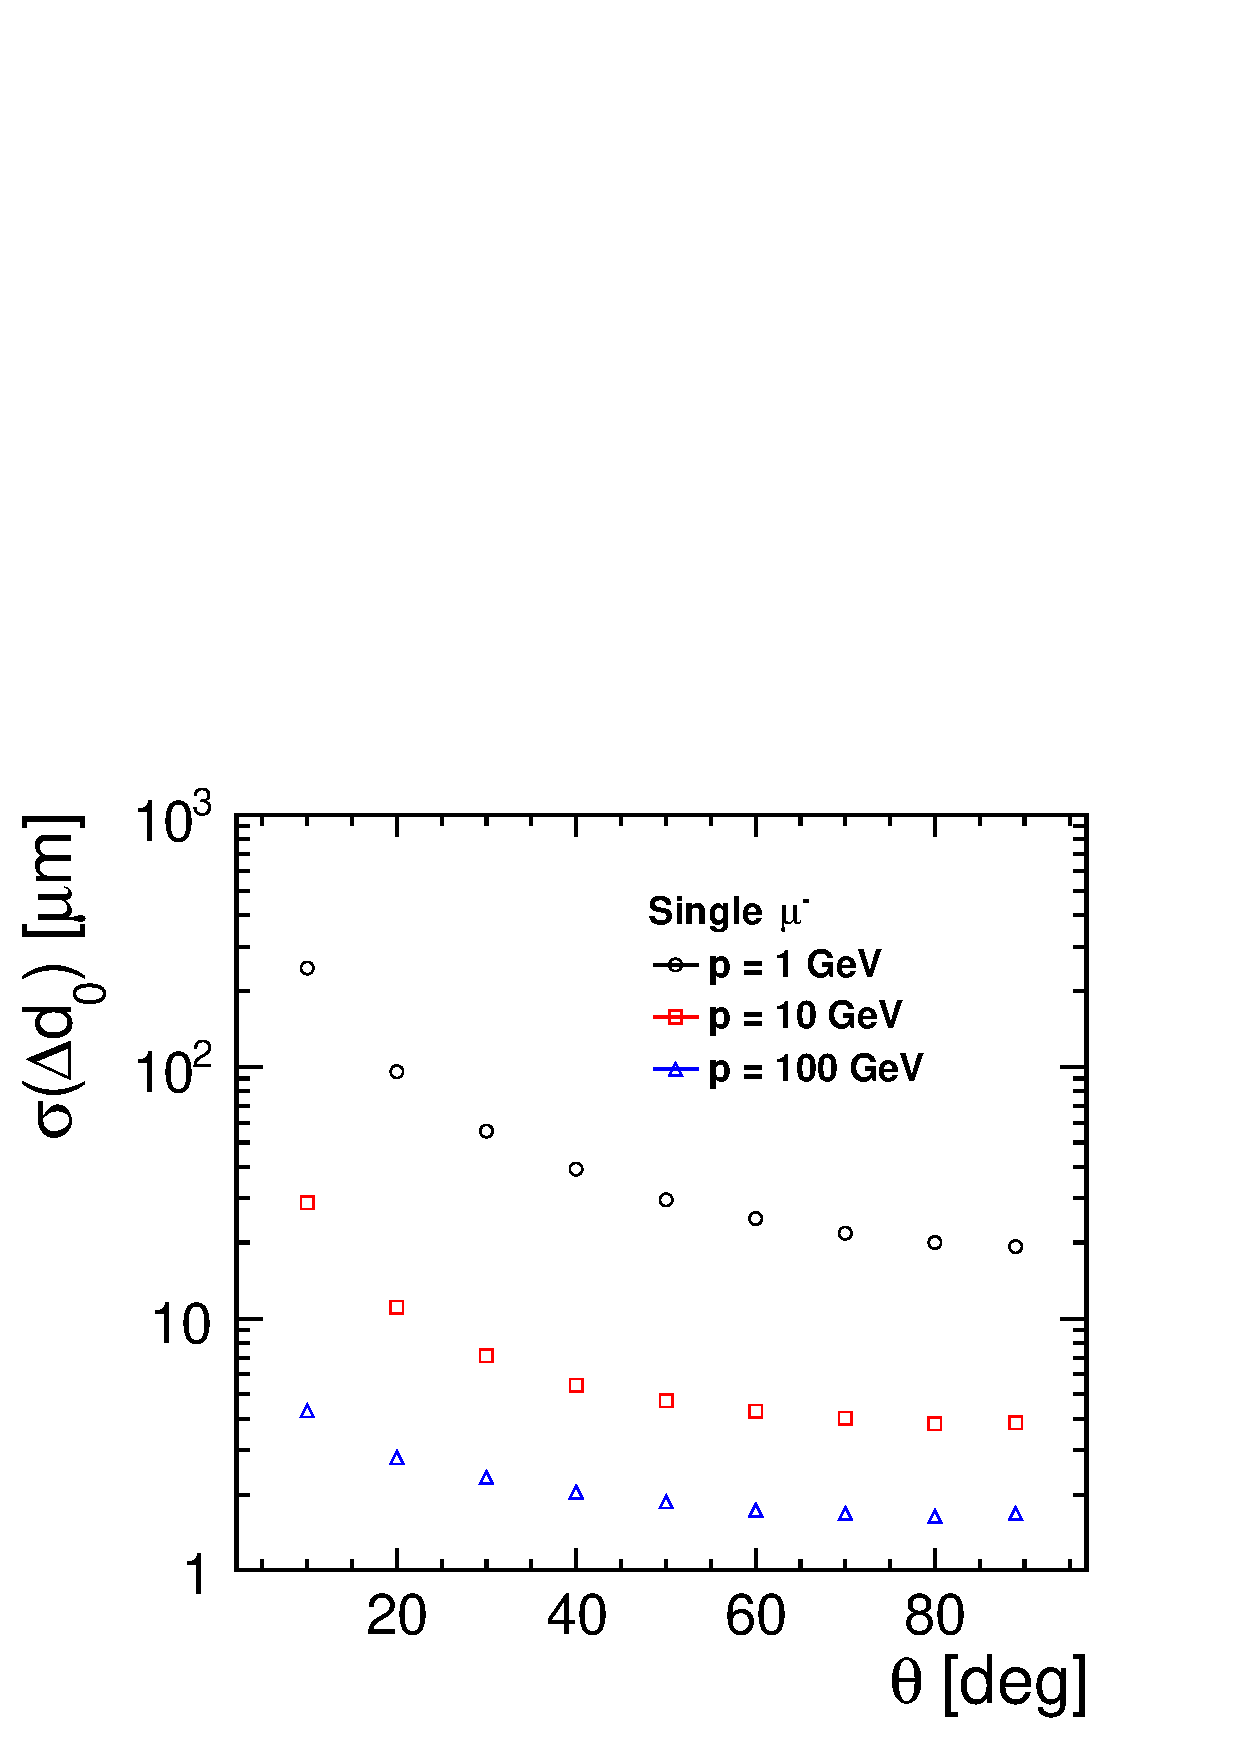
\includegraphics[width=6cm]{../plots_FCCweek_workshop/fromEmilia/d0Res_vs_theta.pdf}};

 \node[inner sep=0pt] (tmp) at (\xRefPosOne-0.2,\yRefPosOne+3.2)
  {\tiny WORK IN PROGRESS};
 \node[inner sep=0pt] (tmp) at (\xRefPosOne+5.99,\yRefPosOne+3.2)
  {\tiny WORK IN PROGRESS};
  
 \node  at (\xRefPosOne+1,\yRefPosOne+4.5) (box){%
    \begin{minipage}{\textwidth}
      \begin{itemize}
		\item Statistics used: 10k single muons at fixed energy and $\theta$ for each datapoint
      \end{itemize}
    \end{minipage}
  };
  
 \node  at (\xRefPosOne+1,\yRefPosOne-2.5) (box){%
    \begin{minipage}{\textwidth}
      \begin{itemize}
		\item Achieved resolutions for 100 GeV muons in the barrel 
		\begin{itemize}
		 \item momentum resolution: 4x10$^{-5}$ GeV$^{-1}$ 
		 \item transverse impact parameter resolution: $<$ 1$\upmu$m
		\end{itemize}
      \end{itemize}
    \end{minipage}
  };
 
 
 

  
\end{tikzpicture}
\end{frame}
%*****************************************************************************
%*****************************************************************************
\begin{frame}{\large \large Tracking efficiency for single muons}
\renewcommand{\yRefPosOne}{-1.5}
\renewcommand{\xRefPosOne}{4.2}
\renewcommand{\xRefIncrementOne}{7.5}
\begin{tikzpicture}[overlay]

 \node[inner sep=0pt] (tmp) at (\xRefPosOne-1.7,\yRefPosOne+0.9)
  {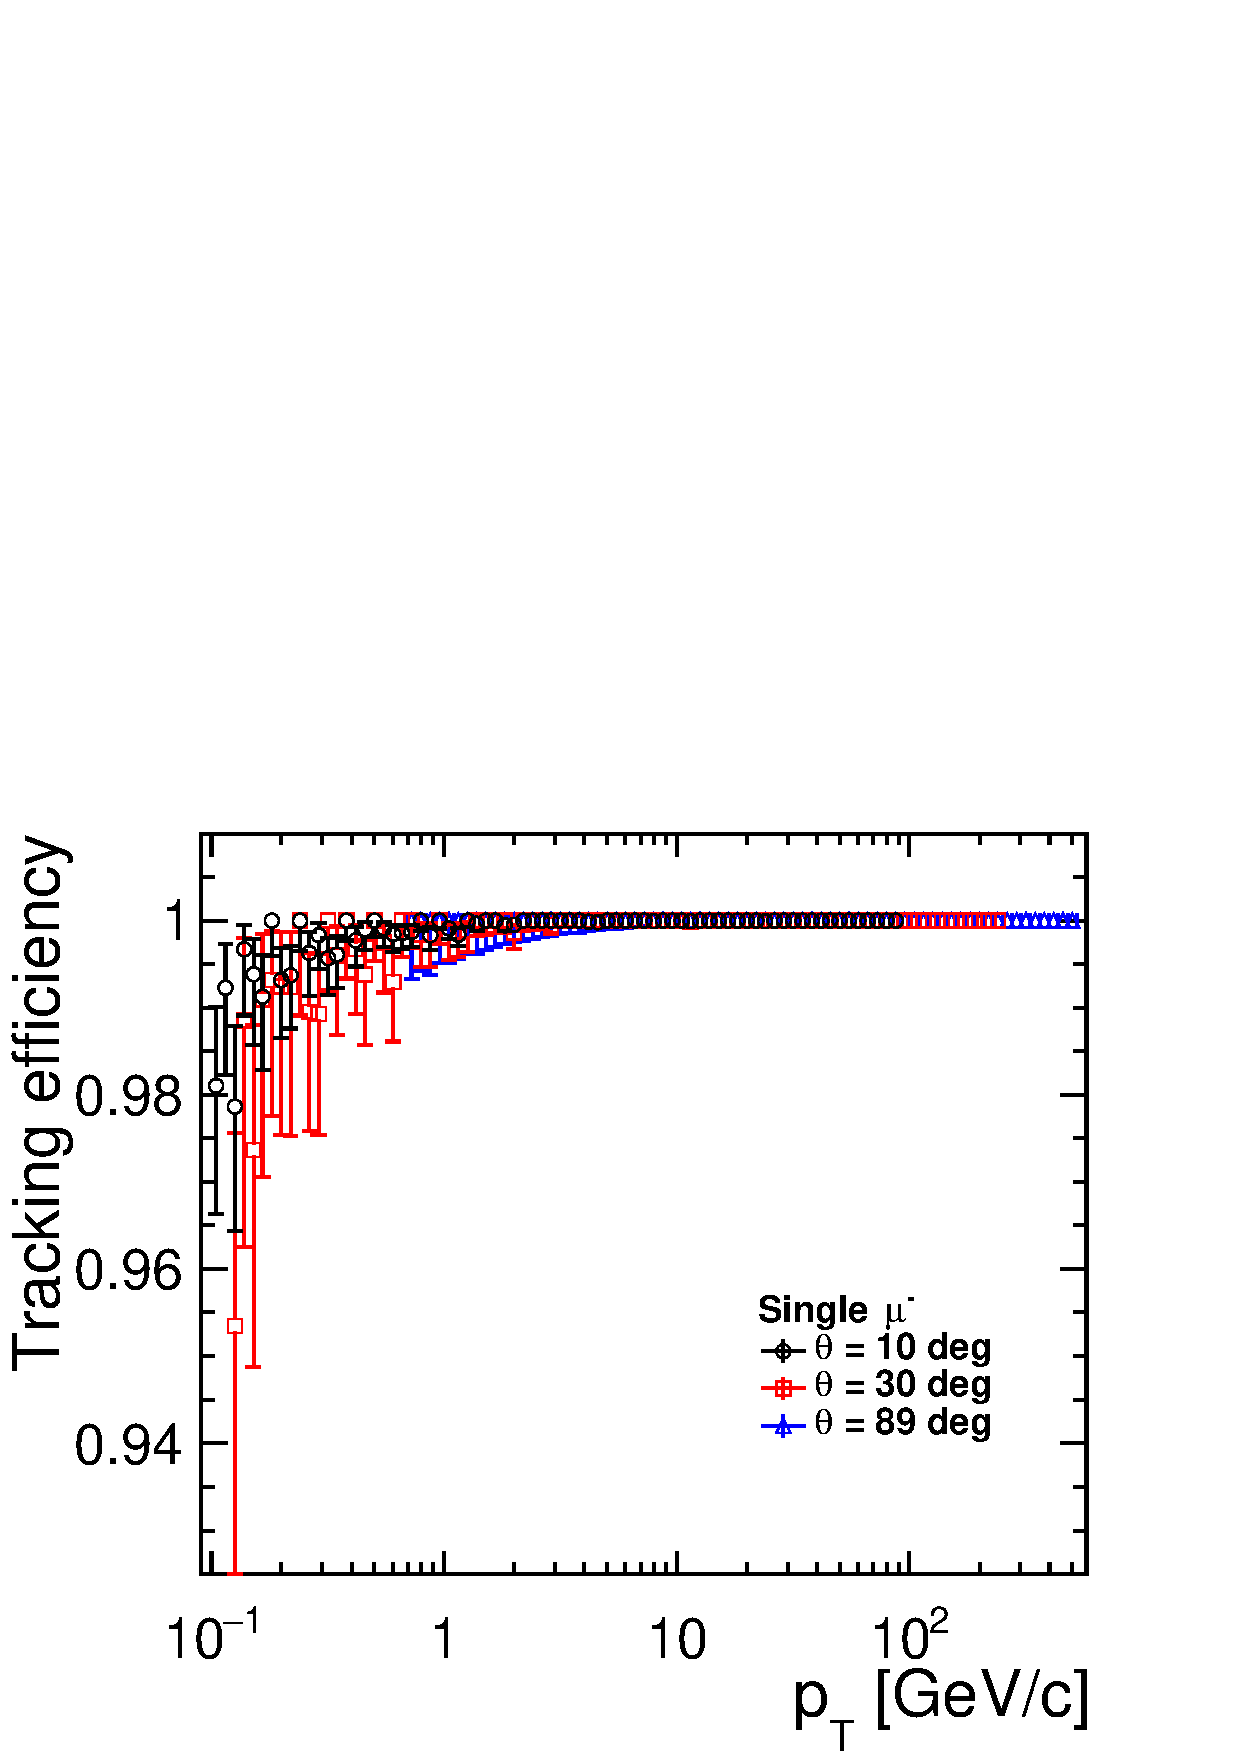
\includegraphics[width=6cm]{../plots_FCCweek_workshop/fromEmilia/eff_vs_pT.pdf}};
  
 \node[inner sep=0pt] (tmp) at (\xRefPosOne+4.5,\yRefPosOne+0.9)
  {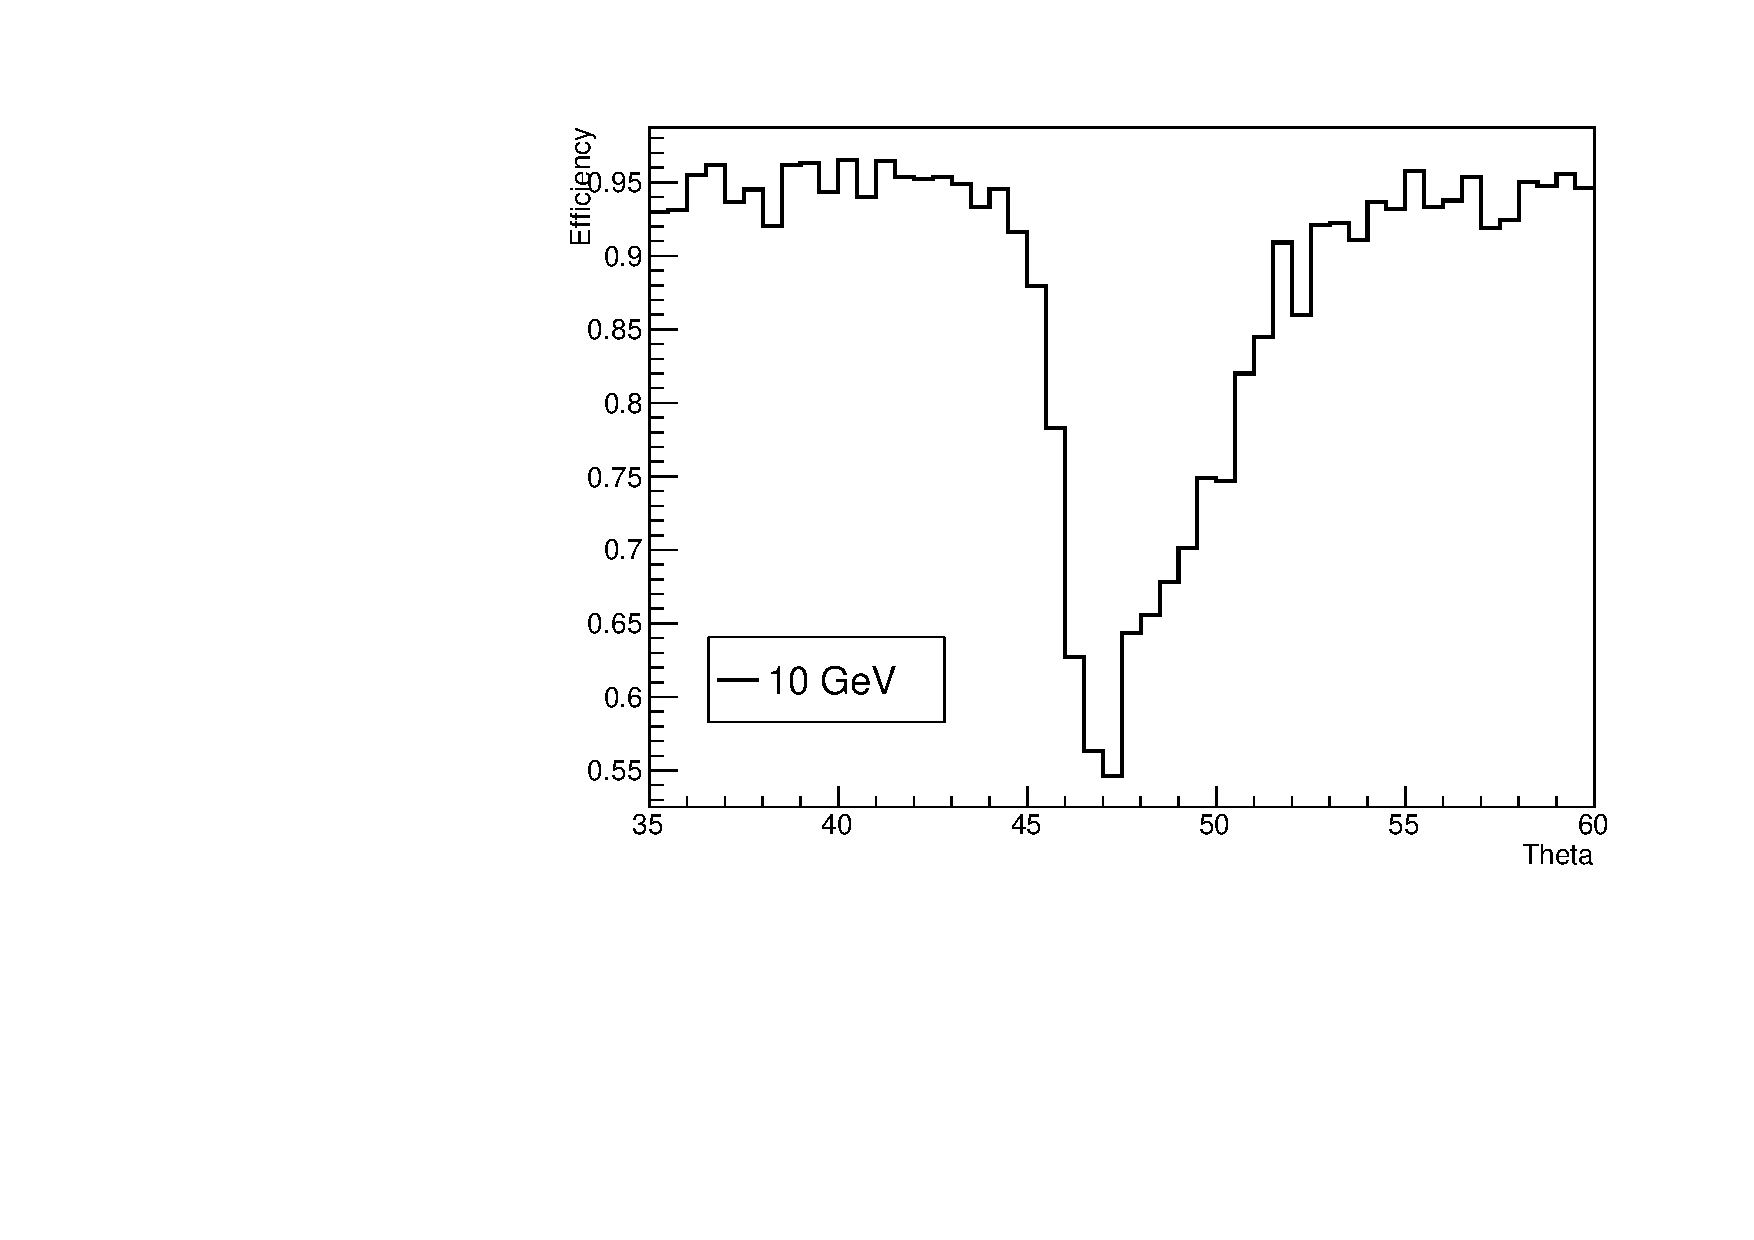
\includegraphics[width=6cm]{../plots_FCCweek_workshop/fromEmilia/eff_vs_theta.pdf}};

 \node[inner sep=0pt] (tmp) at (\xRefPosOne-0.2,\yRefPosOne+3.2)
  {\tiny WORK IN PROGRESS};
 \node[inner sep=0pt] (tmp) at (\xRefPosOne+5.99,\yRefPosOne+3.2)
  {\tiny WORK IN PROGRESS};
  
   \node  at (\xRefPosOne+1,\yRefPosOne+4.2) (box){%
    \begin{minipage}{1.1\textwidth}
      \begin{itemize}
		\item Efficiency = fraction of reconstructed particles out of the reconstructable MC particles
		\item Reconstructable particles: stable MC particles with $p_T >$ 0.1 GeV/c and $|$cos$(\theta)|<0.99$ which left at least 4 unique hits in tracking system
		\item Statistics used: 2M single muons for each dataset
      \end{itemize}
    \end{minipage}
  };
  
 \node  at (\xRefPosOne+1,\yRefPosOne-2.8) (box){%
    \begin{minipage}{\textwidth}
      \begin{itemize}
		\item Fully efficient tracking from 1 GeV
      \end{itemize}
    \end{minipage}
  };
 
 \end{tikzpicture}
\end{frame}
%*****************************************************************************
%*****************************************************************************
\begin{frame}{\large \large Tracking efficiency for Z-like boson events decaying at rest into light quarks}
\renewcommand{\yRefPosOne}{-1.5}
\renewcommand{\xRefPosOne}{4.2}
\renewcommand{\xRefIncrementOne}{7.5}
\begin{tikzpicture}[overlay]

 \node[inner sep=0pt] (tmp) at (\xRefPosOne-1.7,\yRefPosOne+0.9)
  {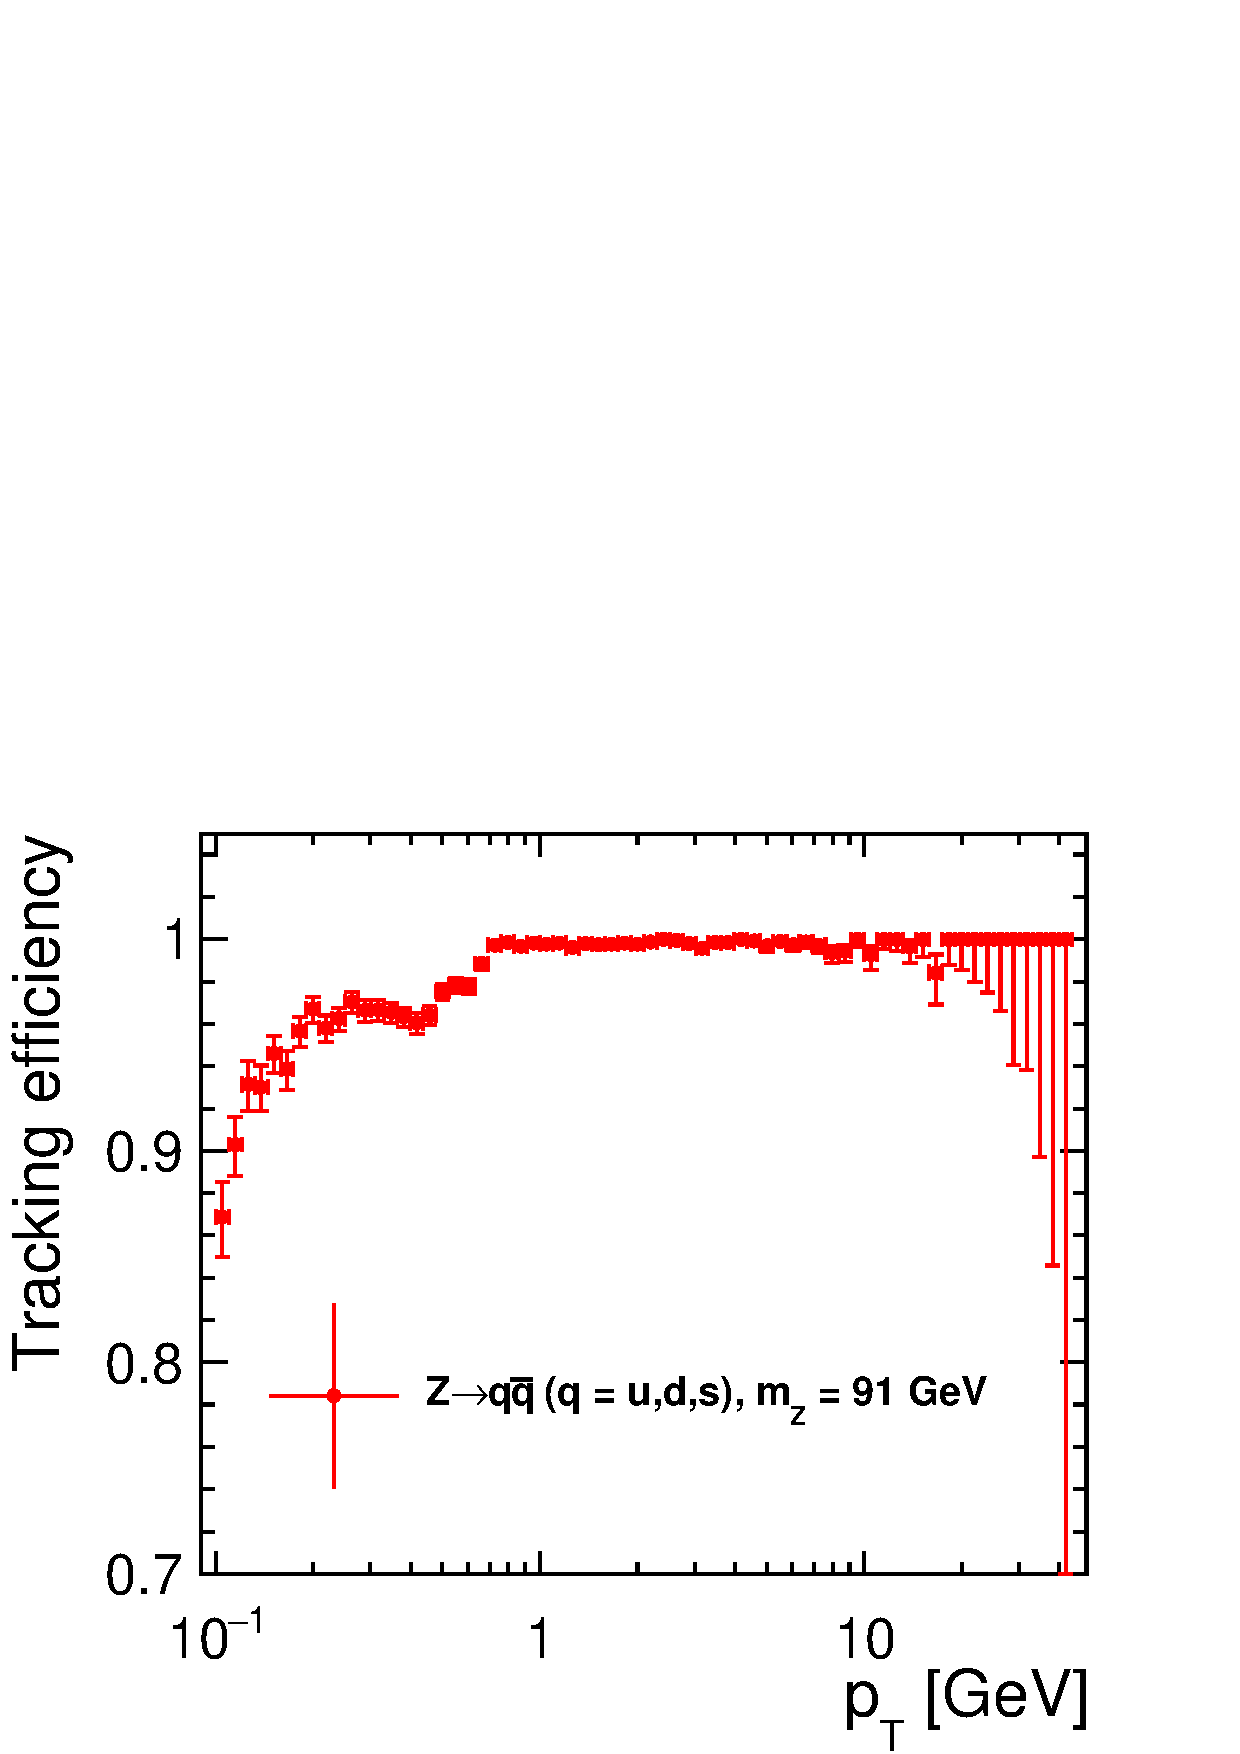
\includegraphics[width=6cm]{../plots_FCCweek_workshop/fromEmilia/eff_vs_pt_91.pdf}};
  
 \node[inner sep=0pt] (tmp) at (\xRefPosOne+4.5,\yRefPosOne+0.9)
  {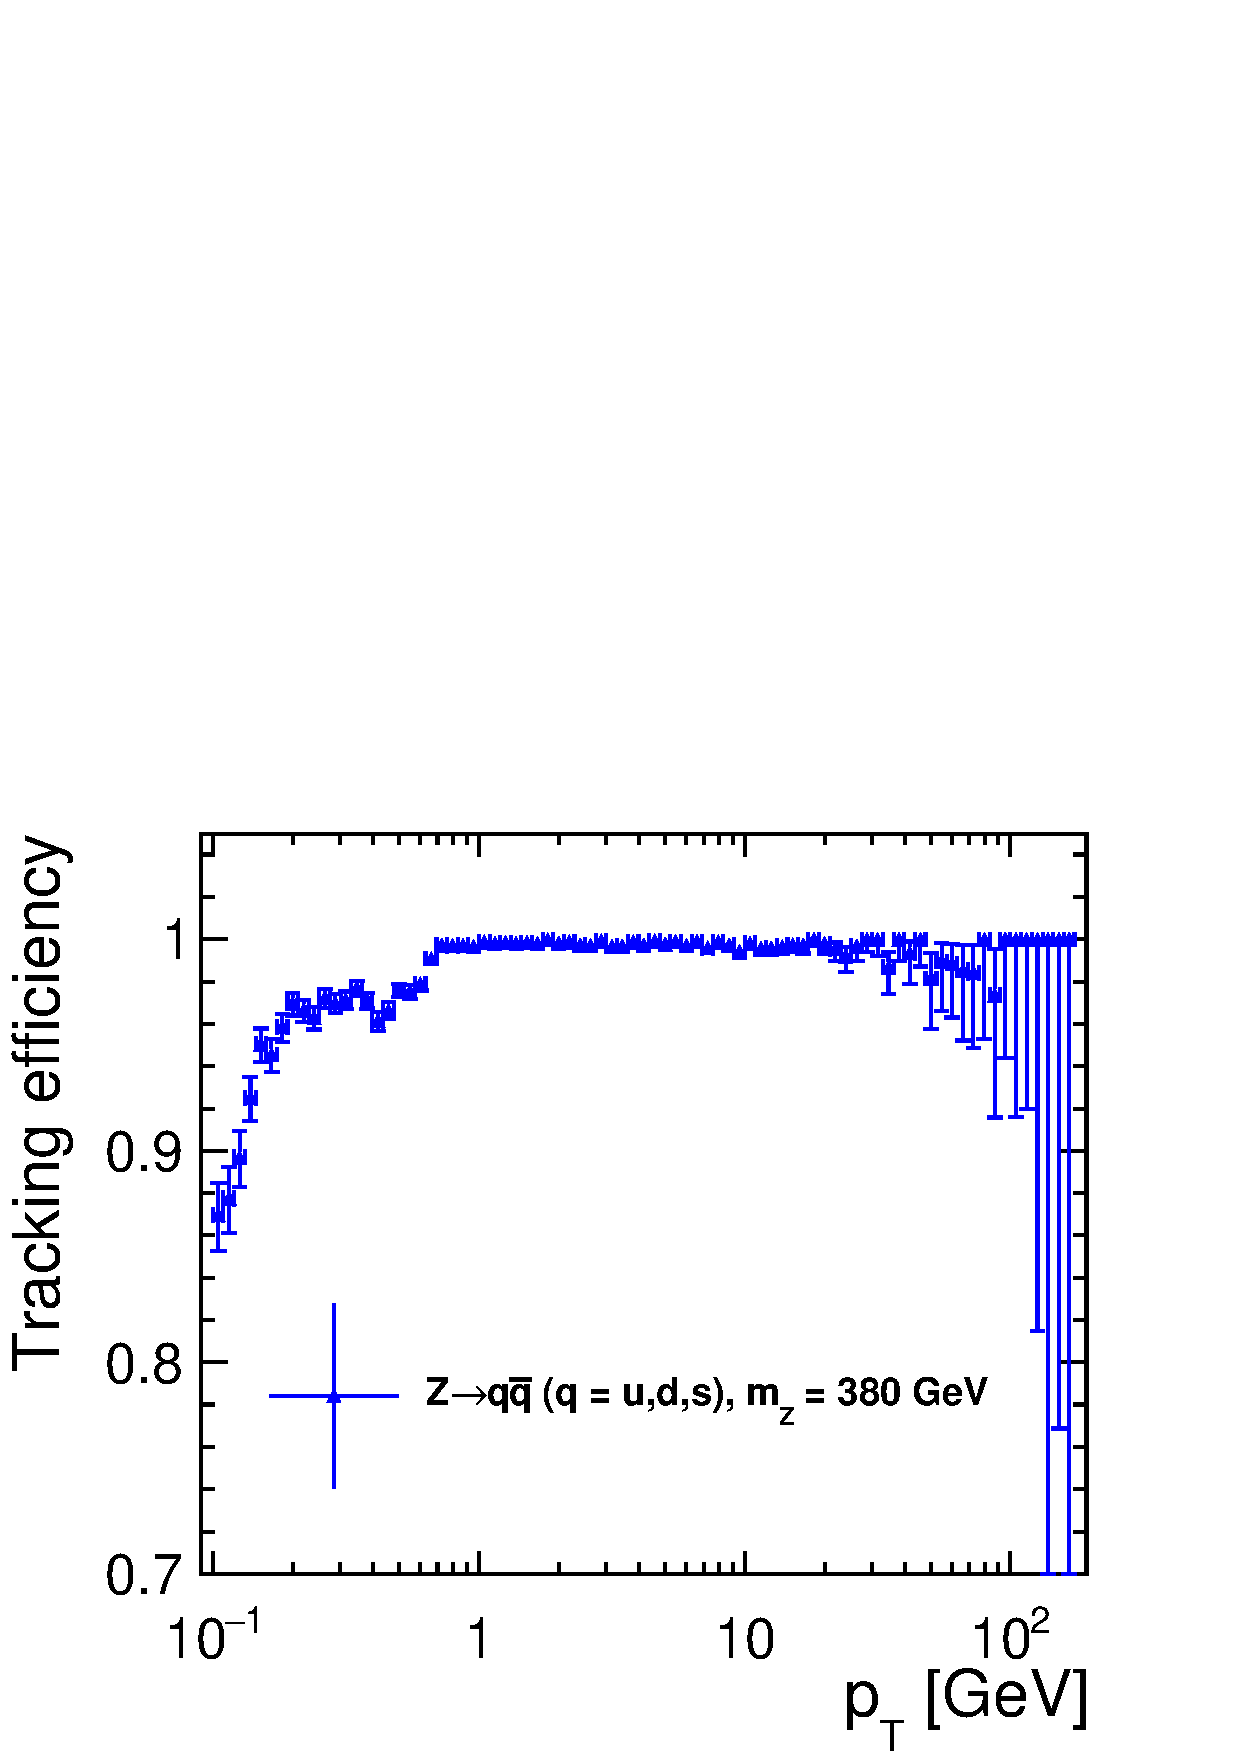
\includegraphics[width=6cm]{../plots_FCCweek_workshop/fromEmilia/eff_vs_pt_380.pdf}};

 \node[inner sep=0pt] (tmp) at (\xRefPosOne-0.2,\yRefPosOne+3.2)
  {\tiny WORK IN PROGRESS};
 \node[inner sep=0pt] (tmp) at (\xRefPosOne+5.99,\yRefPosOne+3.2)
  {\tiny WORK IN PROGRESS};
  
   \node  at (\xRefPosOne+1,\yRefPosOne+4.2) (box){%
    \begin{minipage}{1.1\textwidth}
      \begin{itemize}
		\item Efficiency = fraction of pure reconstructed particles out of the reconstructable MC particles
		\item Pure reconstructed particles: 75$\%$ of hits from track are associated to the simulated MC particle
      \end{itemize}
    \end{minipage}
  };
  
 \node  at (\xRefPosOne+1,\yRefPosOne-2.8) (box){%
    \begin{minipage}{\textwidth}
      \begin{itemize}
		\item Fully efficient tracking from 700 MeV
      \end{itemize}
    \end{minipage}
  };
 
 \end{tikzpicture}
\end{frame}
%*****************************************************************************

%*****************************************************************************
% \bgroup
% \setbeamercolor{background canvas}{bg=white}
\begin{frame}{}

    \begin{tikzpicture}[overlay]

    %% HELPER draw advanced helping grid with axises:
%     \draw (0,-5) to[grid with coordinates] (11,3);

    \node[right] (textNode) at (3,0) {
      { \large \bf Calorimetry performance}
    };
    
    \node[right] (n7) at (4.8,-0.7) {
        \EightStarTaper Single particle identification efficiency 
    };
    
    \node[right] (n8) at (4.8,-1.2) {
        \EightStarTaper Jet energy resolution
    };

%     \node[right] (n9) at (4.6,-1.7) {
%         \EightStarTaper Tracking efficiency in complex events
%     };
    
    \tikz[overlay]\draw[thick,black,->] ([xshift=-0.8cm]textNode.south) to [out=270, in=180] ([xshift=-0.1pt]n7.west);
    \tikz[overlay]\draw[thick,black,->] ([xshift=-1.3cm]textNode.south) to [out=270, in=180] ([xshift=-0.1pt]n8.west);
%     \tikz[overlay]\draw[thick,black,->] ([xshift=-1.8cm]textNode.south) to [out=270, in=180] ([xshift=-0.1pt]n9.west);    

    \end{tikzpicture}

\end{frame}
% \egroup
%*****************************************************************************
%*****************************************************************************
\begin{frame}{\large \large Single particle identification efficiency}
\renewcommand{\yRefPosOne}{-0.9}
\renewcommand{\xRefPosOne}{4.2}
\renewcommand{\xRefIncrementOne}{7.5}
\begin{tikzpicture}[overlay]

 \node[inner sep=0pt] (tmp) at (\xRefPosOne-1.7,\yRefPosOne-0.6)
  {\includegraphics[width=6cm]{/home/oviazlo/Work/Note_FCCeeDetector/figures/CLD_muon_eff.pdf}};
  
 \node[inner sep=0pt] (tmp) at (\xRefPosOne+4.5,\yRefPosOne-0.6)
  {\includegraphics[width=6cm]{/home/oviazlo/Work/Note_FCCeeDetector/figures/CLD_pion_eff.pdf}};


 \node  at (\xRefPosOne+1,\yRefPosOne+3.3) (box){%
    \begin{minipage}{1.1\textwidth}
  \begin{itemize}

   \item Efficiency = fraction or matched reconstructed particles out of the simulated MC particles:
      \begin{itemize}
       \item reconstructed particle of the same type as simulated MC particle
       \item angular matching: $\Delta\theta <$ 1 mrad and $\Delta\phi <$ 2 mrad
       \item energy matching:\\
       - charged particles: $|p_T^{truth} - p_T^{PFO}| < 5\%$ $p_T^{truth} $ \\
       - photons: $\Delta$$E < 5\times\sigma$(ECal) $\approx 0.75\times \sqrt{E}$
      \end{itemize}
    \end{itemize}
    \end{minipage}
  };


  
         \node  at (\xRefPosOne-3.1,\yRefPosOne+1.75) (box){%
    \myCenterBox{\small Muons}
    };     

       \node  at (\xRefPosOne+3,\yRefPosOne+1.75) (box){%
    \myCenterBox{\small Pions}
    };     

 \node[inner sep=0pt] (tmp) at (\xRefPosOne-0.1,\yRefPosOne+1.75)
  {\tiny WORK IN PROGRESS};
 
 \node[inner sep=0pt] (tmp) at (\xRefPosOne+6.1,\yRefPosOne+1.75)
  {\tiny WORK IN PROGRESS};
    
 \node  at (\xRefPosOne+1,\yRefPosOne-3.5) (box){%
    \begin{minipage}{\textwidth}
      \begin{itemize}
        \item $>$99$\%$ muon efficiency and $>$95$\%$ pion efficiency
      \end{itemize}
    \end{minipage}
  };
 
 \end{tikzpicture}
\end{frame}
%*****************************************************************************
%*****************************************************************************
\begin{frame}{\large \large Single particle identification efficiency}
\renewcommand{\yRefPosOne}{-0.5}
\renewcommand{\xRefPosOne}{4.2}
\renewcommand{\xRefIncrementOne}{7.5}
\begin{tikzpicture}[overlay]

 \node[inner sep=0pt] (tmp) at (\xRefPosOne-1.7,\yRefPosOne-0.6)
  {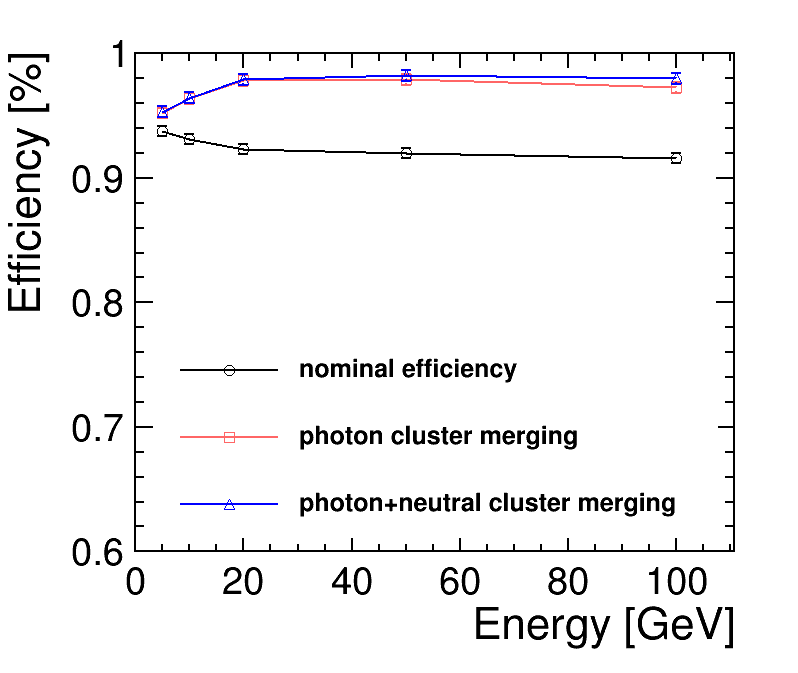
\includegraphics[width=6cm]{/home/oviazlo/Work/Note_FCCeeDetector/figures/calice_photonEff_vs_energy_reclustering_FCCee.pdf}};
  
 \node[inner sep=0pt] (tmp) at (\xRefPosOne+4.5,\yRefPosOne-0.6)
  {\includegraphics[width=6cm]{/home/oviazlo/Work/Note_FCCeeDetector/figures/tempPlots/CLD_electron_eff.pdf}};


 \node  at (\xRefPosOne+1,\yRefPosOne+2.9) (box){%
    \begin{minipage}{1.1\textwidth}
  \begin{itemize}

   \item Photon merging procedure is used to recover inefficiency due to photon conversion
   \item Pandora parameters were retuned in order to recover some electron inefficiency due to Bremsstrahlung
    \end{itemize}
    \end{minipage}
  };


 \node  at (\xRefPosOne+1,\yRefPosOne-3.5) (box){%
    \begin{minipage}{\textwidth}
      \begin{itemize}
        \item $>95\%$ photons and electron efficiency {\tiny [TODO electron plot has to be updated]}
      \end{itemize}
    \end{minipage}
  };
   
       \node  at (\xRefPosOne-3,\yRefPosOne+1.75) (box){%
    \myCenterBox{\small Photons}
    };     

       \node  at (\xRefPosOne+3.25,\yRefPosOne+1.75) (box){%
    \myCenterBox{\small Electrons}
    };     

 \node[inner sep=0pt] (tmp) at (\xRefPosOne-0.1,\yRefPosOne+1.75)
  {\tiny WORK IN PROGRESS};
 
 \node[inner sep=0pt] (tmp) at (\xRefPosOne+6.1,\yRefPosOne+1.75)
  {\tiny WORK IN PROGRESS};
    
 \end{tikzpicture}
\end{frame}
%*****************************************************************************
%*****************************************************************************
\begin{frame}{\large \large Jet Energy Resolution}
\renewcommand{\yRefPosOne}{-0.5}
\renewcommand{\xRefPosOne}{4.2}
\renewcommand{\xRefIncrementOne}{7.5}
\begin{tikzpicture}[overlay]

 \node[inner sep=0pt] (tmp) at (\xRefPosOne-1.7,\yRefPosOne+0.9)
  {\includegraphics[width=6cm]{/home/oviazlo/Work/Note_FCCeeDetector/figures/Sasha_17Jan2018_jet_energy_res.pdf}};
  
 \node[inner sep=0pt] (tmp) at (\xRefPosOne+4.5,\yRefPosOne+0.9)
%   {\includegraphics[width=6cm]{/home/oviazlo/Desktop/beamerPresentations/FCCee/pictures/CEPC_workshop/../oct11_2017/jet_energy.pdf}};
{\includegraphics[width=6cm]{FCCweek/jet_energy.pdf}};
  
 \node[inner sep=0pt] (tmp) at (\xRefPosOne-0.1,\yRefPosOne+3.2)
  {\tiny WORK IN PROGRESS};
 \node[inner sep=0pt] (tmp) at (\xRefPosOne+6.1,\yRefPosOne+3.2)
  {\tiny WORK IN PROGRESS};
  
  
   \node  at (\xRefPosOne+1,\yRefPosOne+3.6) (box){%
    \begin{minipage}{1.1\textwidth}
  \begin{itemize}
   \item Z-like boson events decaying at rest into light quarks (two back-to-back jets)
    \end{itemize}
    \end{minipage}
  };

  
%  \node[inner sep=0pt] (tmp) at (\xRefPosOne+4.5,\yRefPosOne-2.8)
%   {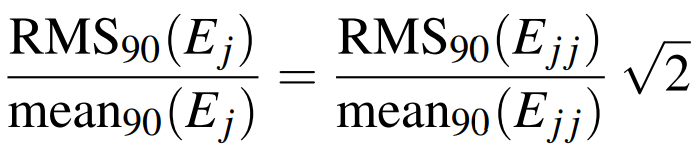
\includegraphics[width=4cm]{/home/oviazlo/Desktop/beamerPresentations/FCCee/pictures/CEPC_workshop/../oct11_2017/jetRes_formula.png}
%   };
%  
  \node[inner sep=0pt] (tmp) at (\xRefPosOne+4.5,\yRefPosOne-3.7)
  {\myCenterBox[yellow]{\href{http://arxiv.org/abs/1209.4039}{arXiv:1209.4039}}  };
 
 
  \node [PixelBox, inner sep=4pt]  at (\xRefPosOne+4.7,\yRefPosOne-2.5) (box){%
    \begin{minipage}{0.45\textwidth}
    \small
		Jet energy (E$_j$) is measured as a half of total energy (E$_{jj}$) of Z$\to$uds di-jet event\\
		
		\hspace{0.4cm}
		  {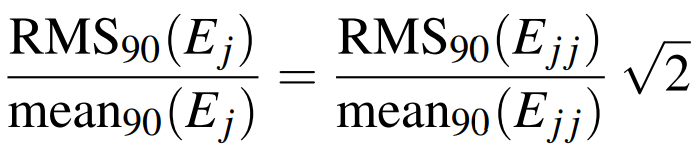
\includegraphics[width=4cm]{/home/oviazlo/Desktop/beamerPresentations/FCCee/pictures/CEPC_workshop/../oct11_2017/jetRes_formula.png}}
		
    \end{minipage}
  };
 
 
 \node  at (\xRefPosOne-0.3,\yRefPosOne-2.8) (box){%
    \begin{minipage}{0.8\textwidth}
      \begin{itemize}
		\item Jet energy resolution in barrel region:
        \begin{itemize}
            \item 45.5 GeV jets: 4-5 $\%$
            \item 190 GeV jets: 3-4 $\%$ \\ [0.2cm]
        \end{itemize}
        \item Total energy is reconstructed with 1$\%$ accuracy:
        \begin{itemize}
            \item 91 GeV: \hspace{0.07cm} 90.4 GeV
            \item 380 GeV: 376.4 GeV
        \end{itemize}
        \item comparable resolution with the CLIC detector 

      \end{itemize}
    \end{minipage}
  };
  
\end{tikzpicture}
\end{frame}
%*****************************************************************************
%*****************************************************************************
\begin{frame}{\large \large Summary and Outlook}
 
 \renewcommand{\yRefPosOne}{0} 
\renewcommand{\xRefPosOne}{5.3}
\renewcommand{\xRefIncrementOne}{5.5}
\begin{tikzpicture}[overlay]

       
\node [TRTBox]  at (\xRefPosOne,\yRefPosOne+2) (box){%
  \begin{minipage}{0.99\textwidth}
  
 \begin{itemize}
  \item The CLD design for the Conceptual Design Report is presented
  \item Tracking and calorimetry performance studies in full simulation demonstrates excellent overall detector performance 
    \end{itemize}
  \end{minipage}
};
\node[fancytitle, right=15pt] at (box.north west) {Summary};

\node [PixelBox] at (\xRefPosOne,\yRefPosOne-2) (box){%
  \begin{minipage}{0.99\textwidth}
  
\begin{itemize}
 \item Further detector performance simulation studies, overlap of incoherent pairs (in progress) and synchrotron radiation backgounds
 \begin{itemize}
  \item If needed optimize timing and/or pT cuts to mitigate impact of background\\[0.3cm]
 \end{itemize}
 \item Full simulation studies of different physics processes 
 \begin{itemize}
  \item software framework and detector model available \\[0.3cm]
 \end{itemize}
 \item Engineering studies
 \begin{itemize}
  \item cooling studies of all subdetectors (no power pulsing)
  \item ECAL optimisation (number of layers, technology choices)
  \item detector opening / maintenance scenarios, impact for detector layout 
 \end{itemize}

\end{itemize}

  
%  \begin{itemize}
%   \item Tracking performance
%   \begin{itemize}
%    \item Momentum resolution and track reconstruction efficiency
%   \end{itemize}
%   \item Calorimetry performance
%   \begin{itemize}
%    \item Single particle ID efficiency 
%    \item Jet energy resolution
%   \end{itemize}
%     \end{itemize}
    
  \end{minipage}
};
\node[fancytitle, right=15pt] at (box.north west) {Outlook};

\node[right] (textNode) at (3,-4.5) {
      { \large \bf Thank you for your attention! }
    };

\end{tikzpicture}
  
\end{frame}
%*****************************************************************************
%*****************************************************************************
% \begin{frame}
% \frametitle{Possible additional plots} 
% 
% \renewcommand{\yRefPosOne}{0}
% \renewcommand{\xRefPosOne}{5.3}
% \renewcommand{\xRefIncrementOne}{5.5}
% 
% \begin{tikzpicture}[overlay]
% 
% \node at (\xRefPosOne,\yRefPosOne) (box){%
%   \begin{minipage}{0.99\textwidth}
%    \begin{itemize}
%   \item Tracking performance:
%   \begin{itemize}
%    \item Angular, $d_0$, $z_0$ resolutions
%   \end{itemize}
% 
%   
%   \item Plots with background overlaid: 
%   \begin{itemize}
%    \item tracking efficiency
%    \item signle particle ID efficiency
%    \item jet energy resolution
%   \end{itemize}
% 
%     \end{itemize}
%   \end{minipage}
% };
% 
% %% HELPER draw advanced helping grid with axises:
% % \draw(-0.5,-4) to[grid with coordinates] (11.5,4);
%  
% \end{tikzpicture}
% \end{frame}
%*****************************************************************************
\backupbegin
%*****************************************************************************
\begin{frame}
\frametitle{BACKUP} 
 
\end{frame}
%*****************************************************************************
\backupend

\end{document}

